\PassOptionsToPackage{unicode=true}{hyperref} % options for packages loaded elsewhere
\PassOptionsToPackage{hyphens}{url}
%
\documentclass[]{article}
\usepackage{lmodern}
\usepackage{amssymb,amsmath}
\usepackage{ifxetex,ifluatex}
\usepackage{fixltx2e} % provides \textsubscript
\ifnum 0\ifxetex 1\fi\ifluatex 1\fi=0 % if pdftex
  \usepackage[T1]{fontenc}
  \usepackage[utf8]{inputenc}
  \usepackage{textcomp} % provides euro and other symbols
\else % if luatex or xelatex
  \usepackage{unicode-math}
  \defaultfontfeatures{Ligatures=TeX,Scale=MatchLowercase}
\fi
% use upquote if available, for straight quotes in verbatim environments
\IfFileExists{upquote.sty}{\usepackage{upquote}}{}
% use microtype if available
\IfFileExists{microtype.sty}{%
\usepackage[]{microtype}
\UseMicrotypeSet[protrusion]{basicmath} % disable protrusion for tt fonts
}{}
\IfFileExists{parskip.sty}{%
\usepackage{parskip}
}{% else
\setlength{\parindent}{0pt}
\setlength{\parskip}{6pt plus 2pt minus 1pt}
}
\usepackage{hyperref}
\hypersetup{
            pdftitle={Series of PCA for Covid-19 study},
            pdfauthor={Matt Blanchard},
            pdfborder={0 0 0},
            breaklinks=true}
\urlstyle{same}  % don't use monospace font for urls
\usepackage[margin=1in]{geometry}
\usepackage{graphicx,grffile}
\makeatletter
\def\maxwidth{\ifdim\Gin@nat@width>\linewidth\linewidth\else\Gin@nat@width\fi}
\def\maxheight{\ifdim\Gin@nat@height>\textheight\textheight\else\Gin@nat@height\fi}
\makeatother
% Scale images if necessary, so that they will not overflow the page
% margins by default, and it is still possible to overwrite the defaults
% using explicit options in \includegraphics[width, height, ...]{}
\setkeys{Gin}{width=\maxwidth,height=\maxheight,keepaspectratio}
\setlength{\emergencystretch}{3em}  % prevent overfull lines
\providecommand{\tightlist}{%
  \setlength{\itemsep}{0pt}\setlength{\parskip}{0pt}}
\setcounter{secnumdepth}{5}
% Redefines (sub)paragraphs to behave more like sections
\ifx\paragraph\undefined\else
\let\oldparagraph\paragraph
\renewcommand{\paragraph}[1]{\oldparagraph{#1}\mbox{}}
\fi
\ifx\subparagraph\undefined\else
\let\oldsubparagraph\subparagraph
\renewcommand{\subparagraph}[1]{\oldsubparagraph{#1}\mbox{}}
\fi

% set default figure placement to htbp
\makeatletter
\def\fps@figure{htbp}
\makeatother

\usepackage{caption}
\captionsetup{labelsep = newline}
\captionsetup{justification = centering, singlelinecheck = false}
\usepackage{pdflscape}
\newcommand{\blandscape}{\begin{landscape}}
\newcommand{\elandscape}{\end{landscape}}
\usepackage{booktabs}
\usepackage{longtable}
\usepackage{array}
\usepackage{multirow}
\usepackage{wrapfig}
\usepackage{float}
\usepackage{colortbl}
\usepackage{pdflscape}
\usepackage{tabu}
\usepackage{threeparttable}
\usepackage{threeparttablex}
\usepackage[normalem]{ulem}
\usepackage{makecell}
\usepackage{xcolor}

\title{Series of PCA for Covid-19 study}
\author{Matt Blanchard}
\date{}

\begin{document}
\maketitle

\hypertarget{summary}{%
\section{Summary}\label{summary}}

I reran all EFAs using the reduced sample (N=1361). The factor
structures were the same, however, there were some minor differences in
the item loadings.\\
1. PCA on Coping, adaptability, resilience, personality, and others.\\
Same 6 factors with minor differences in item loadings\\
- PC2 distraction (+) and acceptance (+) also load\\
- PC3 acceptance (+) also loads\\
- PC4 coping\_denial (+) also loads\\
- PC5 emotionsupp (+) also loads\\
- PC6 cope\_religion (-) loads instead of cope\_reframing (+)\\
2. PCA on coping\\
- PC4 distraction (+) also loads\\
3. Reason\\
- PC1 item 2 (-) also loads\\
- PC3 item 1 (+) also loads

Also, there were a few minor differences and potential issues:\\
4. For the coping variables, I had to use PCA not FA using PAF (poor
fit).\\
5. For the opinion variables, should items 5, 6, or 10 be reverse coded?
When I calculate Cronbach's Alpha it says these items are negatively
correlated with the total scale.

\newpage

\hypertarget{coping-adaptability-reslience-and-personality}{%
\section{Coping, adaptability, reslience, and
personality}\label{coping-adaptability-reslience-and-personality}}

\hypertarget{correlations-between-variables}{%
\subsection{Correlations between
variables}\label{correlations-between-variables}}

\begin{table}

\caption{\label{tab:unnamed-chunk-3}Correlations between variables}
\centering
\resizebox{\linewidth}{!}{
\fontsize{6}{8}\selectfont
\begin{tabular}[t]{llllllllllllllllllllllllllll}
\toprule
  & 1 & 2 & 3 & 4 & 5 & 6 & 7 & 8 & 9 & 10 & 11 & 12 & 13 & 14 & 15 & 16 & 17 & 18 & 19 & 20 & 21 & 22 & 23 & 24 & 25 & 26 & 27\\
\midrule
1. cope\_distraction &  &  &  &  &  &  &  &  &  &  &  &  &  &  &  &  &  &  &  &  &  &  &  &  &  &  & \\
2. cope\_active & .23** &  &  &  &  &  &  &  &  &  &  &  &  &  &  &  &  &  &  &  &  &  &  &  &  &  & \\
3. cope\_denial & .12** & .03 &  &  &  &  &  &  &  &  &  &  &  &  &  &  &  &  &  &  &  &  &  &  &  &  & \\
4. cope\_substance & .10** & .01 & .24** &  &  &  &  &  &  &  &  &  &  &  &  &  &  &  &  &  &  &  &  &  &  &  & \\
5. cope\_emotsupp & .29** & .27** & .14** & .18** &  &  &  &  &  &  &  &  &  &  &  &  &  &  &  &  &  &  &  &  &  &  & \\
\addlinespace
6. cope\_instrsupp & .30** & .27** & .18** & .14** & .74** &  &  &  &  &  &  &  &  &  &  &  &  &  &  &  &  &  &  &  &  &  & \\
7. cope\_disengage & .08** & -.11** & .39** & .32** & .15** & .21** &  &  &  &  &  &  &  &  &  &  &  &  &  &  &  &  &  &  &  &  & \\
8. cope\_venting & .23** & .10** & .30** & .24** & .43** & .48** & .37** &  &  &  &  &  &  &  &  &  &  &  &  &  &  &  &  &  &  &  & \\
9. cope\_reframing & .23** & .42** & .07** & .01 & .24** & .22** & -.06* & .11** &  &  &  &  &  &  &  &  &  &  &  &  &  &  &  &  &  &  & \\
10. cope\_planning & .29** & .52** & .07* & .06* & .36** & .40** & .04 & .29** & .39** &  &  &  &  &  &  &  &  &  &  &  &  &  &  &  &  &  & \\
\addlinespace
11. cope\_humor & .15** & .05 & .09** & .18** & .13** & .11** & .11** & .22** & .23** & .10** &  &  &  &  &  &  &  &  &  &  &  &  &  &  &  &  & \\
12. cope\_acceptance & .17** & .29** & -.23** & -.07** & .12** & .05 & -.21** & -.06* & .29** & .26** & .11** &  &  &  &  &  &  &  &  &  &  &  &  &  &  &  & \\
13. cope\_religion & .05 & .21** & .11** & -.05 & .14** & .22** & .04 & .14** & .24** & .18** & -.03 & .02 &  &  &  &  &  &  &  &  &  &  &  &  &  &  & \\
14. cope\_selfblame & .17** & -.02 & .32** & .29** & .27** & .32** & .50** & .49** & .05 & .25** & .17** & -.14** & .06* &  &  &  &  &  &  &  &  &  &  &  &  &  & \\
15. extraversion & .07** & .15** & .06* & .13** & .19** & .15** & -.02 & .07** & .16** & .08** & .05 & .02 & .07* & -.04 &  &  &  &  &  &  &  &  &  &  &  &  & \\
\addlinespace
16. agreeableness & .18** & .15** & -.05 & -.01 & .25** & .21** & -.10** & .07* & .16** & .11** & -.06* & .11** & .04 & -.01 & .37** &  &  &  &  &  &  &  &  &  &  &  & \\
17. conscientious & -.03 & .18** & -.10** & -.15** & -.06* & -.09** & -.27** & -.20** & .13** & .05 & -.16** & .12** & .08** & -.23** & .02 & .09** &  &  &  &  &  &  &  &  &  &  & \\
18. neuroticism & .17** & -.10** & .16** & .16** & .20** & .20** & .32** & .34** & -.06* & .06* & .01 & -.11** & -.02 & .40** & -.09** & .05 & -.24** &  &  &  &  &  &  &  &  &  & \\
19. intellect & .10** & .12** & -.11** & -.02 & .12** & .09** & -.08** & .07** & .11** & .16** & .06* & .14** & .02 & .01 & .13** & .23** & -.02 & .01 &  &  &  &  &  &  &  &  & \\
20. resilience & .01 & .29** & -.08** & -.10** & -.02 & -.06* & -.36** & -.21** & .28** & .14** & .06* & .24** & .06* & -.32** & .26** & .12** & .31** & -.51** & .14** &  &  &  &  &  &  &  & \\
\addlinespace
21. adaptability\_crisis & -.06* & .22** & -.09** & -.03 & -.03 & -.06* & -.20** & -.17** & .15** & .12** & .01 & .20** & .05 & -.22** & .22** & .06* & .23** & -.34** & .11** & .60** &  &  &  &  &  &  & \\
22. adaptability\_uncertainty & -.06* & .21** & -.15** & -.06* & -.05 & -.09** & -.28** & -.21** & .16** & .09** & .01 & .22** & .00 & -.28** & .26** & .16** & .18** & -.44** & .20** & .64** & .68** &  &  &  &  &  & \\
23. conservatism & -.02 & .11** & .10** & -.08** & -.09** & -.10** & -.08** & -.13** & .10** & .00 & -.05 & -.01 & .13** & -.15** & .10** & -.07* & .14** & -.13** & -.16** & .19** & .14** & .05 &  &  &  &  & \\
24. reactance & -.03 & -.06* & .18** & .18** & .00 & -.01 & .24** & .19** & -.01 & .02 & .14** & -.11** & -.02 & .17** & .02 & -.21** & -.23** & .16** & .02 & -.07* & -.01 & -.07** & .02 &  &  &  & \\
25. gov\_trust & -.07* & .03 & -.02 & -.07* & -.05 & -.06* & -.14** & -.16** & .09** & -.04 & -.07* & .04 & .07** & -.14** & .08** & .00 & .15** & -.10** & -.07* & .14** & .05 & .08** & .29** & -.14** &  &  & \\
\addlinespace
26. cultural\_tightloose & .08** & .03 & -.01 & -.04 & -.01 & -.01 & -.04 & -.05 & .07** & -.01 & .01 & .10** & -.02 & -.04 & -.03 & .03 & .06* & -.02 & -.04 & .06* & .05 & .00 & .13** & .00 & .07** &  & \\
27. RWA & .03 & .09** & .17** & -.08** & -.07* & -.03 & .02 & -.05 & .11** & .00 & -.10** & -.04 & .14** & -.08** & .07* & -.09** & .16** & -.03 & -.23** & .09** & .06* & -.03 & .52** & -.02 & .22** & .18** & \\
28. PoliticalOrient & .08** & -.07* & -.01 & .11** & .14** & .15** & .10** & .13** & -.04 & .02 & .06* & .00 & -.12** & .14** & -.01 & .15** & -.13** & .12** & .16** & -.13** & -.12** & -.05 & -.47** & .00 & -.28** & -.06* & -.39**\\
\bottomrule
\end{tabular}}
\end{table}

\hypertarget{kmo-and-bartletts-test-of-spherecity}{%
\subsection{KMO and Bartlett's test of
spherecity}\label{kmo-and-bartletts-test-of-spherecity}}

\begin{table}[H]

\caption{\label{tab:unnamed-chunk-4}KMO: Measure of sampling adequacy}
\centering
\fontsize{6}{8}\selectfont
\begin{tabular}[t]{r}
\toprule
KMO\\
\midrule
0.82\\
\bottomrule
\end{tabular}
\end{table}

\begin{table}[H]

\caption{\label{tab:unnamed-chunk-4}Bartletts test of spherecity}
\centering
\fontsize{6}{8}\selectfont
\begin{tabular}[t]{rrr}
\toprule
chisq & p.value & df\\
\midrule
9949 & 0 & 378\\
\bottomrule
\end{tabular}
\end{table}

\hypertarget{scree-plot}{%
\subsection{Scree plot}\label{scree-plot}}

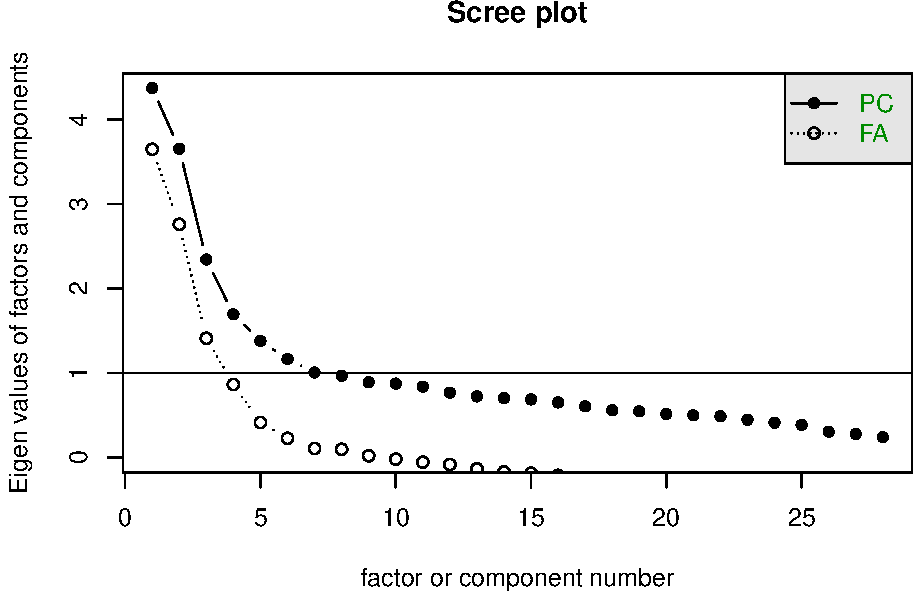
\includegraphics{PCA_covid_files/figure-latex/unnamed-chunk-5-1.pdf}

The scree plot suggests a 6 or 7 component solution. SK extracted 6
components from the full dataset so I will do the same.

\hypertarget{pca-6-components}{%
\subsection{PCA: 6 components}\label{pca-6-components}}

\begin{table}[H]

\caption{\label{tab:unnamed-chunk-6}Variance accounted for by components}
\centering
\fontsize{6}{8}\selectfont
\begin{tabular}[t]{rrlll}
\toprule
component & eigen & prop\_var & cum\_var & rotation\_SS\_load\\
\midrule
1 & 4.37 & 0.11 & 0.11 & 3.1\\
2 & 3.65 & 0.11 & 0.22 & 3.1\\
3 & 2.34 & 0.11 & 0.33 & 2.96\\
4 & 1.69 & 0.09 & 0.42 & 2.49\\
5 & 1.38 & 0.06 & 0.48 & 1.67\\
\addlinespace
6 & 1.17 & 0.05 & 0.52 & 1.29\\
7 & 1.01 &  &  & \\
8 & 0.97 &  &  & \\
9 & 0.89 &  &  & \\
10 & 0.87 &  &  & \\
\addlinespace
11 & 0.84 &  &  & \\
12 & 0.77 &  &  & \\
13 & 0.72 &  &  & \\
14 & 0.70 &  &  & \\
15 & 0.69 &  &  & \\
\addlinespace
16 & 0.65 &  &  & \\
17 & 0.61 &  &  & \\
18 & 0.56 &  &  & \\
19 & 0.55 &  &  & \\
20 & 0.52 &  &  & \\
\addlinespace
21 & 0.50 &  &  & \\
22 & 0.49 &  &  & \\
23 & 0.45 &  &  & \\
24 & 0.41 &  &  & \\
25 & 0.39 &  &  & \\
\addlinespace
26 & 0.31 &  &  & \\
27 & 0.28 &  &  & \\
28 & 0.24 &  &  & \\
\bottomrule
\end{tabular}
\end{table}

\begin{table}[H]

\caption{\label{tab:unnamed-chunk-6}Pattern Matrix}
\centering
\fontsize{6}{8}\selectfont
\begin{tabular}[t]{lllllllr}
\toprule
var & PC1 & PC2 & PC3 & PC4 & PC5 & PC6 & h2\\
\midrule
adaptability\_uncertainty & 0.87 &  &  &  &  &  & 0.73\\
adaptability\_crisis & 0.84 &  &  &  &  &  & 0.64\\
resilience & 0.8 &  &  &  &  &  & 0.73\\
extraversion & 0.44 &  &  &  & 0.71 &  & 0.62\\
neuroticism & -0.6 &  &  &  &  &  & 0.50\\
\addlinespace
cope\_planning &  & 0.8 &  &  &  &  & 0.60\\
cope\_active &  & 0.71 &  &  &  &  & 0.55\\
cope\_instrsupp &  & 0.6 &  &  &  &  & 0.65\\
cope\_reframing &  & 0.6 &  &  &  &  & 0.49\\
cope\_emotsupp &  & 0.54 &  &  & 0.33 &  & 0.61\\
\addlinespace
cope\_religion &  & 0.52 &  &  &  & -0.4 & 0.42\\
cope\_acceptance &  & 0.4 & -0.34 &  &  & 0.45 & 0.53\\
cope\_venting &  & 0.39 & 0.49 &  &  &  & 0.57\\
cope\_distraction &  & 0.35 &  &  &  & 0.44 & 0.43\\
cope\_disengage &  &  & 0.68 &  &  &  & 0.55\\
\addlinespace
cope\_denial &  &  & 0.65 & 0.31 &  &  & 0.47\\
reactance &  &  & 0.65 &  &  &  & 0.42\\
cope\_substance &  &  & 0.62 &  &  &  & 0.39\\
cope\_selfblame &  &  & 0.54 &  &  &  & 0.54\\
cope\_humor &  &  & 0.42 &  &  & 0.44 & 0.44\\
\addlinespace
conscientious &  &  & -0.41 &  &  &  & 0.33\\
RWA &  &  &  & 0.82 &  &  & 0.61\\
conservatism &  &  &  & 0.8 &  &  & 0.62\\
gov\_trust &  &  &  & 0.5 &  &  & 0.31\\
cultural\_tightloose &  &  &  & 0.37 &  & 0.63 & 0.42\\
\addlinespace
PoliticalOrient &  &  &  & -0.67 &  &  & 0.49\\
intellect &  &  &  & -0.39 &  &  & 0.29\\
agreeableness &  &  &  &  & 0.8 &  & 0.67\\
\bottomrule
\end{tabular}
\end{table}

\begin{table}[H]

\caption{\label{tab:unnamed-chunk-6}Correlations between components}
\centering
\fontsize{6}{8}\selectfont
\begin{tabular}[t]{lrrrrrr}
\toprule
  & RC1 & RC2 & RC4 & RC3 & RC5 & RC6\\
\midrule
RC1 & 1.00 & -0.01 & -0.35 & 0.15 & -0.11 & 0.19\\
RC2 & -0.01 & 1.00 & 0.15 & -0.03 & 0.32 & 0.11\\
RC4 & -0.35 & 0.15 & 1.00 & -0.20 & 0.15 & 0.00\\
RC3 & 0.15 & -0.03 & -0.20 & 1.00 & -0.09 & -0.19\\
RC5 & -0.11 & 0.32 & 0.15 & -0.09 & 1.00 & -0.04\\
\addlinespace
RC6 & 0.19 & 0.11 & 0.00 & -0.19 & -0.04 & 1.00\\
\bottomrule
\end{tabular}
\end{table}

\newpage

\hypertarget{biz-statements}{%
\section{Biz statements}\label{biz-statements}}

\hypertarget{correlations-between-variables-1}{%
\subsection{Correlations between
variables}\label{correlations-between-variables-1}}

\begin{table}[H]

\caption{\label{tab:unnamed-chunk-7}Correlations between variables}
\centering
\fontsize{6}{8}\selectfont
\begin{tabular}[t]{llll}
\toprule
  & 1 & 2 & 3\\
\midrule
1. WFH\_Biz\_Statements\_1 &  &  & \\
2. WFH\_Biz\_Statements\_2 & .44** &  & \\
3. WFH\_Biz\_Statements\_3 & .24* & .31** & \\
4. WFH\_Biz\_Statements\_4 & .33** & .53** & .64**\\
\bottomrule
\end{tabular}
\end{table}

\hypertarget{reliability}{%
\subsection{Reliability}\label{reliability}}

\begin{table}[H]

\caption{\label{tab:unnamed-chunk-8}Cronbach's Alpha}
\centering
\fontsize{6}{8}\selectfont
\begin{tabular}[t]{r}
\toprule
a\\
\midrule
0.72\\
\bottomrule
\end{tabular}
\end{table}

\hypertarget{kmo-and-bartletts-test-of-spherecity-1}{%
\subsection{KMO and Bartlett's test of
spherecity}\label{kmo-and-bartletts-test-of-spherecity-1}}

\begin{table}[H]

\caption{\label{tab:unnamed-chunk-9}KMO: Measure of sampling adequacy}
\centering
\fontsize{6}{8}\selectfont
\begin{tabular}[t]{r}
\toprule
KMO\\
\midrule
0.65\\
\bottomrule
\end{tabular}
\end{table}

\begin{table}[H]

\caption{\label{tab:unnamed-chunk-9}Bartletts test of spherecity}
\centering
\fontsize{6}{8}\selectfont
\begin{tabular}[t]{rrr}
\toprule
chisq & p.value & df\\
\midrule
88 & 0 & 6\\
\bottomrule
\end{tabular}
\end{table}

\hypertarget{scree-plot-1}{%
\subsection{Scree plot}\label{scree-plot-1}}

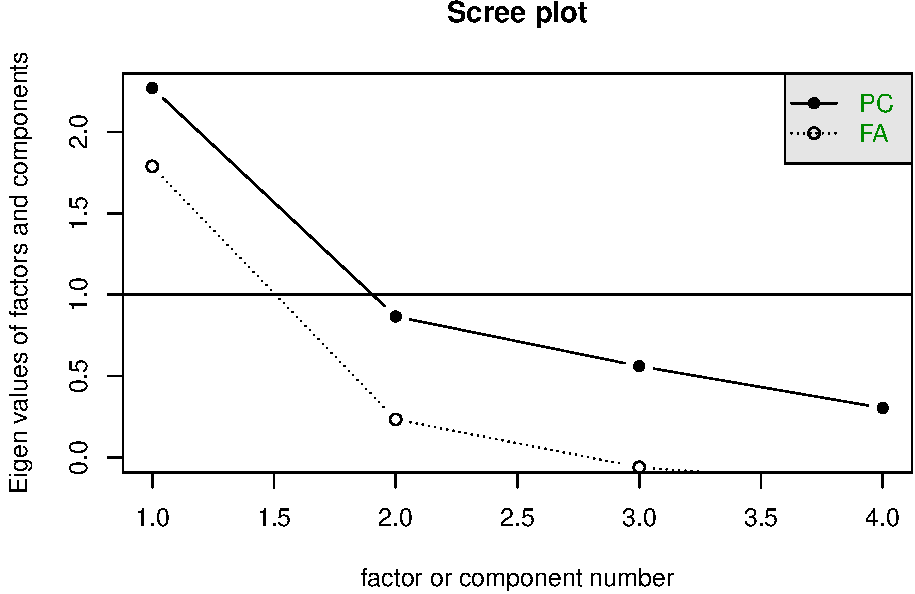
\includegraphics{PCA_covid_files/figure-latex/unnamed-chunk-10-1.pdf}

The scree plot suggests a 1 component solution. This is consistent with
the components extracted by SK from the full dataset.

\hypertarget{pca-1-component}{%
\subsection{PCA: 1 component}\label{pca-1-component}}

\begin{table}[H]

\caption{\label{tab:unnamed-chunk-11}Variance accounted for by components}
\centering
\fontsize{6}{8}\selectfont
\begin{tabular}[t]{rrlll}
\toprule
component & eigen & prop\_var & cum\_var & rotation\_SS\_load\\
\midrule
1 & 2.27 & 0.57 & 0.57 & 2.27\\
2 & 0.87 &  &  & \\
3 & 0.56 &  &  & \\
4 & 0.30 &  &  & \\
\bottomrule
\end{tabular}
\end{table}

\begin{table}[H]

\caption{\label{tab:unnamed-chunk-11}Pattern Matrix}
\centering
\fontsize{6}{8}\selectfont
\begin{tabular}[t]{lrr}
\toprule
var & PC1 & h2\\
\midrule
WFH\_Biz\_Statements\_4 & 0.86 & 0.74\\
WFH\_Biz\_Statements\_2 & 0.76 & 0.58\\
WFH\_Biz\_Statements\_3 & 0.74 & 0.55\\
WFH\_Biz\_Statements\_1 & 0.63 & 0.40\\
\bottomrule
\end{tabular}
\end{table}

\newpage

\hypertarget{compliance}{%
\section{Compliance}\label{compliance}}

\hypertarget{correlations-between-variables-2}{%
\subsection{Correlations between
variables}\label{correlations-between-variables-2}}

\begin{table}[H]

\caption{\label{tab:unnamed-chunk-12}Correlations between variables}
\centering
\fontsize{6}{8}\selectfont
\begin{tabular}[t]{llllllllllll}
\toprule
  & 1 & 2 & 3 & 4 & 5 & 6 & 7 & 8 & 9 & 10 & 11\\
\midrule
1. BehaviourComply\_1\_1 &  &  &  &  &  &  &  &  &  &  & \\
2. BehaviourComply\_1\_2 & .25** &  &  &  &  &  &  &  &  &  & \\
3. BehaviourComply\_1\_3 & .47** & .35** &  &  &  &  &  &  &  &  & \\
4. BehaviourComply\_1\_4 & .09** & .20** & .29** &  &  &  &  &  &  &  & \\
5. BehaviourComply\_1\_5 & .06* & .13** & .20** & .38** &  &  &  &  &  &  & \\
\addlinespace
6. BehaviourComply\_1\_6 & .18** & .29** & .38** & .25** & .28** &  &  &  &  &  & \\
7. BehaviourComply\_2\_1 & .42** & .28** & .50** & .27** & .18** & .34** &  &  &  &  & \\
8. BehaviourComply\_2\_2 & .40** & .42** & .50** & .21** & .13** & .41** & .46** &  &  &  & \\
9. BehaviourComply\_2\_3 & .22** & .29** & .28** & .23** & .20** & .31** & .39** & .43** &  &  & \\
10. BehaviourComply\_2\_4 & .13** & .19** & .22** & .28** & .21** & .20** & .29** & .18** & .21** &  & \\
\addlinespace
11. BehaviourComply\_2\_5 & .08** & .07* & .17** & .25** & .21** & .10** & .17** & .08** & .14** & .42** & \\
12. BehaviourComply\_2\_6 & .27** & .19** & .31** & .25** & .20** & .26** & .34** & .21** & .22** & .56** & .39**\\
\bottomrule
\end{tabular}
\end{table}

\hypertarget{reliability-1}{%
\subsection{Reliability}\label{reliability-1}}

\begin{table}[H]

\caption{\label{tab:unnamed-chunk-13}Cronbach's Alpha}
\centering
\fontsize{6}{8}\selectfont
\begin{tabular}[t]{r}
\toprule
a\\
\midrule
0.79\\
\bottomrule
\end{tabular}
\end{table}

\hypertarget{kmo-and-bartletts-test-of-spherecity-2}{%
\subsection{KMO and Bartlett's test of
spherecity}\label{kmo-and-bartletts-test-of-spherecity-2}}

\begin{table}[H]

\caption{\label{tab:unnamed-chunk-14}KMO: Measure of sampling adequacy}
\centering
\fontsize{6}{8}\selectfont
\begin{tabular}[t]{r}
\toprule
KMO\\
\midrule
0.85\\
\bottomrule
\end{tabular}
\end{table}

\begin{table}[H]

\caption{\label{tab:unnamed-chunk-14}Bartletts test of spherecity}
\centering
\fontsize{6}{8}\selectfont
\begin{tabular}[t]{rrr}
\toprule
chisq & p.value & df\\
\midrule
4086 & 0 & 66\\
\bottomrule
\end{tabular}
\end{table}

\hypertarget{scree-plot-2}{%
\subsection{Scree plot}\label{scree-plot-2}}

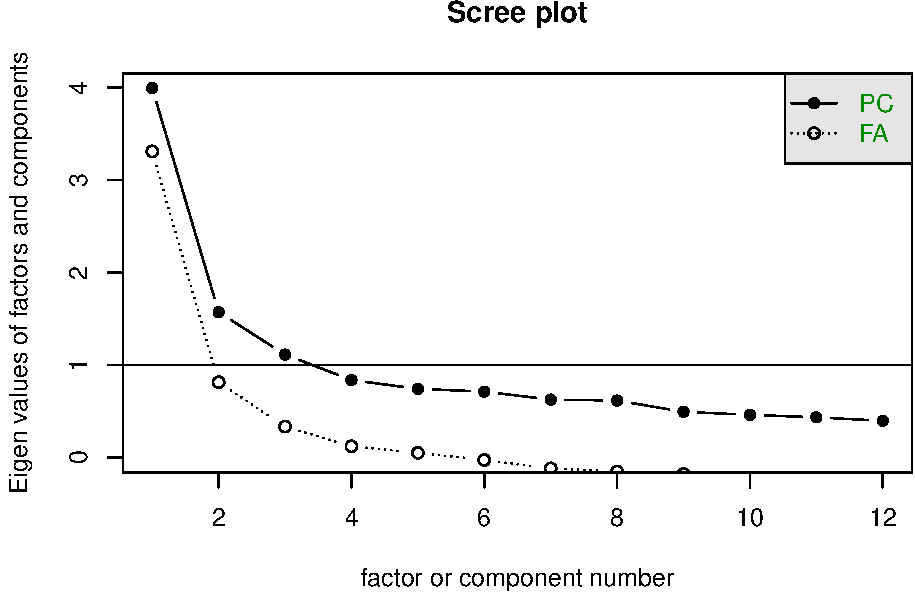
\includegraphics{PCA_covid_files/figure-latex/unnamed-chunk-15-1.pdf}

The scree plot suggests a 3 component solution. This is consistent with
the components extracted by SK from the full dataset.

\hypertarget{pca-3-component}{%
\subsection{PCA: 3 component}\label{pca-3-component}}

\begin{table}[H]

\caption{\label{tab:unnamed-chunk-16}Variance accounted for by components}
\centering
\fontsize{6}{8}\selectfont
\begin{tabular}[t]{rrlll}
\toprule
component & eigen & prop\_var & cum\_var & rotation\_SS\_load\\
\midrule
1 & 4.00 & 0.26 & 0.26 & 3.12\\
2 & 1.57 & 0.16 & 0.42 & 1.93\\
3 & 1.11 & 0.14 & 0.56 & 1.63\\
4 & 0.84 &  &  & \\
5 & 0.74 &  &  & \\
\addlinespace
6 & 0.71 &  &  & \\
7 & 0.63 &  &  & \\
8 & 0.62 &  &  & \\
9 & 0.49 &  &  & \\
10 & 0.46 &  &  & \\
\addlinespace
11 & 0.43 &  &  & \\
12 & 0.40 &  &  & \\
\bottomrule
\end{tabular}
\end{table}

\begin{table}[H]

\caption{\label{tab:unnamed-chunk-16}Pattern Matrix}
\centering
\fontsize{6}{8}\selectfont
\begin{tabular}[t]{llllr}
\toprule
var & PC1 & PC2 & PC3 & h2\\
\midrule
BehaviourComply\_2\_2 & 0.82 &  &  & 0.64\\
BehaviourComply\_1\_1 & 0.79 &  & -0.42 & 0.59\\
BehaviourComply\_1\_3 & 0.73 &  &  & 0.58\\
BehaviourComply\_2\_1 & 0.69 &  &  & 0.55\\
BehaviourComply\_1\_2 & 0.58 &  &  & 0.37\\
\addlinespace
BehaviourComply\_2\_3 & 0.49 &  &  & 0.39\\
BehaviourComply\_1\_6 & 0.42 &  & 0.43 & 0.47\\
BehaviourComply\_2\_4 &  & 0.77 &  & 0.66\\
BehaviourComply\_2\_5 &  & 0.76 &  & 0.58\\
BehaviourComply\_2\_6 &  & 0.76 &  & 0.68\\
\addlinespace
BehaviourComply\_1\_5 &  &  & 0.83 & 0.63\\
BehaviourComply\_1\_4 &  &  & 0.69 & 0.55\\
\bottomrule
\end{tabular}
\end{table}

\begin{table}[H]

\caption{\label{tab:unnamed-chunk-16}Correlations between components}
\centering
\fontsize{6}{8}\selectfont
\begin{tabular}[t]{lrrr}
\toprule
  & RC1 & RC2 & RC3\\
\midrule
RC1 & 1.0 & 0.30 & 0.40\\
RC2 & 0.3 & 1.00 & 0.27\\
RC3 & 0.4 & 0.27 & 1.00\\
\bottomrule
\end{tabular}
\end{table}

\newpage

\hypertarget{coping}{%
\section{Coping}\label{coping}}

\hypertarget{correlations-between-variables-3}{%
\subsection{Correlations between
variables}\label{correlations-between-variables-3}}

\begin{table}[H]

\caption{\label{tab:unnamed-chunk-17}Correlations between variables}
\centering
\fontsize{6}{8}\selectfont
\begin{tabular}[t]{llllllllllllll}
\toprule
  & 1 & 2 & 3 & 4 & 5 & 6 & 7 & 8 & 9 & 10 & 11 & 12 & 13\\
\midrule
1. cope\_distraction &  &  &  &  &  &  &  &  &  &  &  &  & \\
2. cope\_active & .23** &  &  &  &  &  &  &  &  &  &  &  & \\
3. cope\_denial & .12** & .03 &  &  &  &  &  &  &  &  &  &  & \\
4. cope\_substance & .10** & .01 & .24** &  &  &  &  &  &  &  &  &  & \\
5. cope\_emotsupp & .29** & .27** & .14** & .18** &  &  &  &  &  &  &  &  & \\
\addlinespace
6. cope\_instrsupp & .30** & .27** & .18** & .14** & .74** &  &  &  &  &  &  &  & \\
7. cope\_disengage & .08** & -.11** & .39** & .32** & .15** & .21** &  &  &  &  &  &  & \\
8. cope\_venting & .23** & .10** & .30** & .24** & .43** & .48** & .37** &  &  &  &  &  & \\
9. cope\_reframing & .23** & .42** & .07** & .01 & .24** & .22** & -.06* & .11** &  &  &  &  & \\
10. cope\_planning & .29** & .52** & .07* & .06* & .36** & .40** & .04 & .29** & .39** &  &  &  & \\
\addlinespace
11. cope\_humor & .15** & .05 & .09** & .18** & .13** & .11** & .11** & .22** & .23** & .10** &  &  & \\
12. cope\_acceptance & .17** & .29** & -.23** & -.07** & .12** & .05 & -.21** & -.06* & .29** & .26** & .11** &  & \\
13. cope\_religion & .05 & .21** & .11** & -.05 & .14** & .22** & .04 & .14** & .24** & .18** & -.03 & .02 & \\
14. cope\_selfblame & .17** & -.02 & .32** & .29** & .27** & .32** & .50** & .49** & .05 & .25** & .17** & -.14** & .06*\\
\bottomrule
\end{tabular}
\end{table}

\hypertarget{reliability-2}{%
\subsection{Reliability}\label{reliability-2}}

\begin{table}[H]

\caption{\label{tab:unnamed-chunk-18}Cronbach's Alpha}
\centering
\fontsize{6}{8}\selectfont
\begin{tabular}[t]{r}
\toprule
a\\
\midrule
0.75\\
\bottomrule
\end{tabular}
\end{table}

\hypertarget{kmo-and-bartletts-test-of-spherecity-3}{%
\subsection{KMO and Bartlett's test of
spherecity}\label{kmo-and-bartletts-test-of-spherecity-3}}

\begin{table}[H]

\caption{\label{tab:unnamed-chunk-19}KMO: Measure of sampling adequacy}
\centering
\fontsize{6}{8}\selectfont
\begin{tabular}[t]{r}
\toprule
KMO\\
\midrule
0.79\\
\bottomrule
\end{tabular}
\end{table}

\begin{table}[H]

\caption{\label{tab:unnamed-chunk-19}Bartletts test of spherecity}
\centering
\fontsize{6}{8}\selectfont
\begin{tabular}[t]{rrr}
\toprule
chisq & p.value & df\\
\midrule
4644 & 0 & 91\\
\bottomrule
\end{tabular}
\end{table}

\hypertarget{scree-plot-3}{%
\subsection{Scree plot}\label{scree-plot-3}}

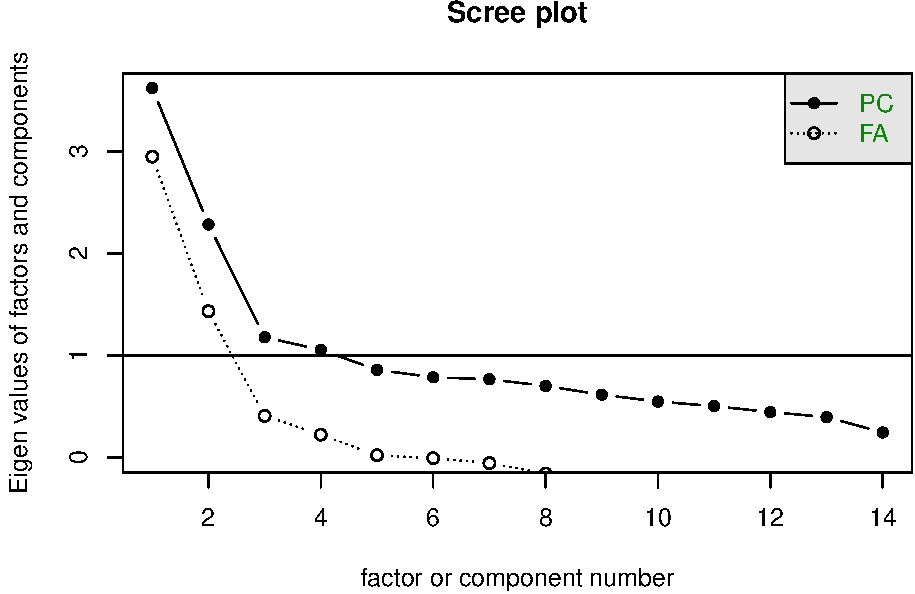
\includegraphics{PCA_covid_files/figure-latex/unnamed-chunk-20-1.pdf}

The scree plot suggests either a 2 factor (FA) solution or a 4 component
(PCA) solution. SK extracted 4 factors using PAF from the full dataset.
I will conduct a 4 component PCA.

\hypertarget{pca-4-components}{%
\subsection{PCA: 4 components}\label{pca-4-components}}

\begin{table}[H]

\caption{\label{tab:unnamed-chunk-21}Variance accounted for by components}
\centering
\fontsize{6}{8}\selectfont
\begin{tabular}[t]{rrlll}
\toprule
component & eigen & prop\_var & cum\_var & rotation\_SS\_load\\
\midrule
1 & 3.62 & 0.17 & 0.17 & 2.37\\
2 & 2.28 & 0.17 & 0.34 & 2.33\\
3 & 1.18 & 0.15 & 0.49 & 2.12\\
4 & 1.05 & 0.09 & 0.58 & 1.32\\
5 & 0.86 &  &  & \\
\addlinespace
6 & 0.79 &  &  & \\
7 & 0.77 &  &  & \\
8 & 0.70 &  &  & \\
9 & 0.61 &  &  & \\
10 & 0.55 &  &  & \\
\addlinespace
11 & 0.50 &  &  & \\
12 & 0.45 &  &  & \\
13 & 0.40 &  &  & \\
14 & 0.25 &  &  & \\
\bottomrule
\end{tabular}
\end{table}

\begin{table}[H]

\caption{\label{tab:unnamed-chunk-21}Pattern Matrix}
\centering
\fontsize{6}{8}\selectfont
\begin{tabular}[t]{lllllr}
\toprule
var & PC1 & PC2 & PC3 & PC4 & h2\\
\midrule
cope\_instrsupp & 0.93 &  &  &  & 0.79\\
cope\_emotsupp & 0.92 &  &  &  & 0.75\\
cope\_venting & 0.53 & 0.42 &  &  & 0.59\\
cope\_planning & 0.36 &  & 0.52 &  & 0.56\\
cope\_distraction & 0.33 &  &  &  & 0.34\\
\addlinespace
cope\_denial &  & 0.76 &  &  & 0.55\\
cope\_disengage &  & 0.73 &  &  & 0.59\\
cope\_selfblame &  & 0.6 &  &  & 0.56\\
cope\_substance &  & 0.46 &  & 0.47 & 0.42\\
cope\_acceptance &  & -0.51 & 0.33 & 0.35 & 0.55\\
\addlinespace
cope\_reframing &  &  & 0.81 &  & 0.64\\
cope\_active &  &  & 0.69 &  & 0.58\\
cope\_religion &  &  & 0.66 & -0.51 & 0.64\\
cope\_humor &  &  &  & 0.77 & 0.57\\
\bottomrule
\end{tabular}
\end{table}

\begin{table}[H]

\caption{\label{tab:unnamed-chunk-21}Correlations between components}
\centering
\fontsize{6}{8}\selectfont
\begin{tabular}[t]{lrrrr}
\toprule
  & RC1 & RC2 & RC4 & RC3\\
\midrule
RC1 & 1.00 & 0.25 & 0.40 & 0.38\\
RC2 & 0.25 & 1.00 & -0.05 & 0.04\\
RC4 & 0.40 & -0.05 & 1.00 & 0.16\\
RC3 & 0.38 & 0.04 & 0.16 & 1.00\\
\bottomrule
\end{tabular}
\end{table}

\newpage

\hypertarget{dass}{%
\section{DASS}\label{dass}}

\hypertarget{correlations-between-variables-4}{%
\subsection{Correlations between
variables}\label{correlations-between-variables-4}}

\begin{table}[H]

\caption{\label{tab:unnamed-chunk-22}Correlations between variables}
\centering
\fontsize{6}{8}\selectfont
\begin{tabular}[t]{lll}
\toprule
  & 1 & 2\\
\midrule
1. DASS\_stress &  & \\
2. DASS\_anxiety & .79** & \\
3. DASS\_depression & .71** & .68**\\
\bottomrule
\end{tabular}
\end{table}

\hypertarget{reliability-3}{%
\subsection{Reliability}\label{reliability-3}}

\begin{table}[H]

\caption{\label{tab:unnamed-chunk-23}Cronbach's Alpha}
\centering
\fontsize{6}{8}\selectfont
\begin{tabular}[t]{r}
\toprule
a\\
\midrule
0.88\\
\bottomrule
\end{tabular}
\end{table}

\hypertarget{kmo-and-bartletts-test-of-spherecity-4}{%
\subsection{KMO and Bartlett's test of
spherecity}\label{kmo-and-bartletts-test-of-spherecity-4}}

\begin{table}[H]

\caption{\label{tab:unnamed-chunk-24}KMO: Measure of sampling adequacy}
\centering
\fontsize{6}{8}\selectfont
\begin{tabular}[t]{r}
\toprule
KMO\\
\midrule
0.73\\
\bottomrule
\end{tabular}
\end{table}

\begin{table}[H]

\caption{\label{tab:unnamed-chunk-24}Bartletts test of spherecity}
\centering
\fontsize{6}{8}\selectfont
\begin{tabular}[t]{rrr}
\toprule
chisq & p.value & df\\
\midrule
286 & 0 & 3\\
\bottomrule
\end{tabular}
\end{table}

\hypertarget{scree-plot-4}{%
\subsection{Scree plot}\label{scree-plot-4}}

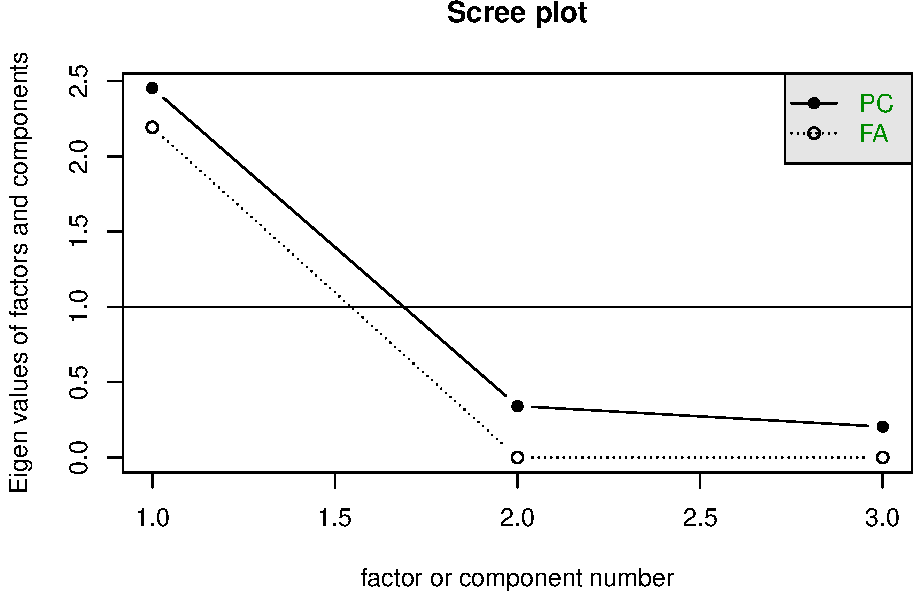
\includegraphics{PCA_covid_files/figure-latex/unnamed-chunk-25-1.pdf}

\hypertarget{pca}{%
\subsection{PCA}\label{pca}}

The scree plot suggests a 1 component solution. This is consistent with
the components extracted by SK from the full dataset.

\hypertarget{pca-1-component-1}{%
\subsection{PCA: 1 component}\label{pca-1-component-1}}

\begin{table}[H]

\caption{\label{tab:unnamed-chunk-26}Variance accounted for by components}
\centering
\fontsize{6}{8}\selectfont
\begin{tabular}[t]{rrlll}
\toprule
component & eigen & prop\_var & cum\_var & rotation\_SS\_load\\
\midrule
1 & 2.45 & 0.82 & 0.82 & 2.45\\
2 & 0.34 &  &  & \\
3 & 0.20 &  &  & \\
\bottomrule
\end{tabular}
\end{table}

\begin{table}[H]

\caption{\label{tab:unnamed-chunk-26}Pattern Matrix}
\centering
\fontsize{6}{8}\selectfont
\begin{tabular}[t]{lrr}
\toprule
var & PC1 & h2\\
\midrule
DASS\_stress & 0.92 & 0.85\\
DASS\_anxiety & 0.91 & 0.83\\
DASS\_depression & 0.88 & 0.77\\
\bottomrule
\end{tabular}
\end{table}

\newpage

\hypertarget{follow}{%
\section{Follow}\label{follow}}

\hypertarget{correlations-between-variables-5}{%
\subsection{Correlations between
variables}\label{correlations-between-variables-5}}

\begin{table}[H]

\caption{\label{tab:unnamed-chunk-27}Correlations between variables}
\centering
\fontsize{6}{8}\selectfont
\begin{tabular}[t]{llll}
\toprule
  & 1 & 2 & 3\\
\midrule
1. follow\_self &  &  & \\
2. follow\_family & .68** &  & \\
3. follow\_atrisk & .60** & .73** & \\
4. follow\_people & .66** & .69** & .78**\\
\bottomrule
\end{tabular}
\end{table}

\hypertarget{reliability-4}{%
\subsection{Reliability}\label{reliability-4}}

\begin{table}[H]

\caption{\label{tab:unnamed-chunk-28}Cronbach's Alpha}
\centering
\fontsize{6}{8}\selectfont
\begin{tabular}[t]{r}
\toprule
a\\
\midrule
0.9\\
\bottomrule
\end{tabular}
\end{table}

\hypertarget{kmo-and-bartletts-test-of-spherecity-5}{%
\subsection{KMO and Bartlett's test of
spherecity}\label{kmo-and-bartletts-test-of-spherecity-5}}

\begin{table}[H]

\caption{\label{tab:unnamed-chunk-29}KMO: Measure of sampling adequacy}
\centering
\fontsize{6}{8}\selectfont
\begin{tabular}[t]{r}
\toprule
KMO\\
\midrule
0.81\\
\bottomrule
\end{tabular}
\end{table}

\begin{table}[H]

\caption{\label{tab:unnamed-chunk-29}Bartletts test of spherecity}
\centering
\fontsize{6}{8}\selectfont
\begin{tabular}[t]{rrr}
\toprule
chisq & p.value & df\\
\midrule
3360 & 0 & 6\\
\bottomrule
\end{tabular}
\end{table}

\hypertarget{scree-plot-5}{%
\subsection{Scree plot}\label{scree-plot-5}}

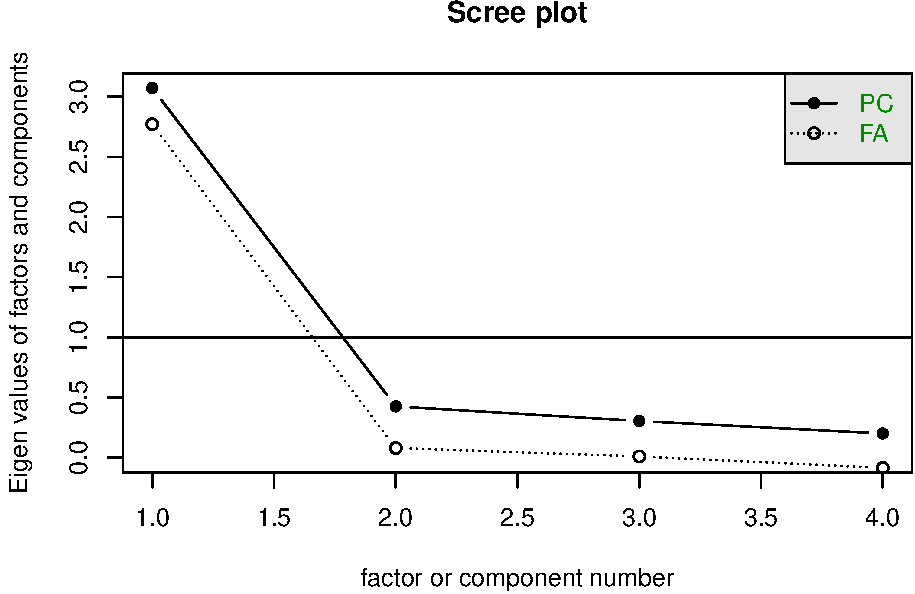
\includegraphics{PCA_covid_files/figure-latex/unnamed-chunk-30-1.pdf}

\hypertarget{pca-1}{%
\subsection{PCA}\label{pca-1}}

The scree plot suggests a 1 component solution. This is consistent with
the components extracted by SK from the full dataset.

\hypertarget{pca-1-component-2}{%
\subsection{PCA: 1 component}\label{pca-1-component-2}}

\begin{table}[H]

\caption{\label{tab:unnamed-chunk-31}Variance accounted for by components}
\centering
\fontsize{6}{8}\selectfont
\begin{tabular}[t]{rrlll}
\toprule
component & eigen & prop\_var & cum\_var & rotation\_SS\_load\\
\midrule
1 & 3.07 & 0.77 & 0.77 & 3.07\\
2 & 0.42 &  &  & \\
3 & 0.30 &  &  & \\
4 & 0.20 &  &  & \\
\bottomrule
\end{tabular}
\end{table}

\begin{table}[H]

\caption{\label{tab:unnamed-chunk-31}Pattern Matrix}
\centering
\fontsize{6}{8}\selectfont
\begin{tabular}[t]{lrr}
\toprule
var & PC1 & h2\\
\midrule
follow\_people & 0.90 & 0.80\\
follow\_family & 0.89 & 0.78\\
follow\_atrisk & 0.89 & 0.79\\
follow\_self & 0.83 & 0.69\\
\bottomrule
\end{tabular}
\end{table}

\newpage

\hypertarget{government}{%
\section{Government}\label{government}}

\hypertarget{correlations-between-variables-6}{%
\subsection{Correlations between
variables}\label{correlations-between-variables-6}}

\begin{table}[H]

\caption{\label{tab:unnamed-chunk-32}Correlations between variables}
\centering
\fontsize{6}{8}\selectfont
\begin{tabular}[t]{lll}
\toprule
  & 1 & 2\\
\midrule
1. Govt\_Satisfaction &  & \\
2. Govt\_Extreme & -.58** & \\
3. Govt\_Truth & .62** & -.35**\\
\bottomrule
\end{tabular}
\end{table}

\hypertarget{reliability-5}{%
\subsection{Reliability}\label{reliability-5}}

\begin{table}[H]

\caption{\label{tab:unnamed-chunk-33}Cronbach's Alpha}
\centering
\fontsize{6}{8}\selectfont
\begin{tabular}[t]{r}
\toprule
a\\
\midrule
0.76\\
\bottomrule
\end{tabular}
\end{table}

\hypertarget{kmo-and-bartletts-test-of-spherecity-6}{%
\subsection{KMO and Bartlett's test of
spherecity}\label{kmo-and-bartletts-test-of-spherecity-6}}

\begin{table}[H]

\caption{\label{tab:unnamed-chunk-34}KMO: Measure of sampling adequacy}
\centering
\fontsize{6}{8}\selectfont
\begin{tabular}[t]{r}
\toprule
KMO\\
\midrule
0.61\\
\bottomrule
\end{tabular}
\end{table}

\begin{table}[H]

\caption{\label{tab:unnamed-chunk-34}Bartletts test of spherecity}
\centering
\fontsize{6}{8}\selectfont
\begin{tabular}[t]{rrr}
\toprule
chisq & p.value & df\\
\midrule
1192 & 0 & 3\\
\bottomrule
\end{tabular}
\end{table}

\hypertarget{scree-plot-6}{%
\subsection{Scree plot}\label{scree-plot-6}}

An ultra-Heywood case was detected for FA so I only plotted eigen values
using PCA here. This issue did not occur for PCA.

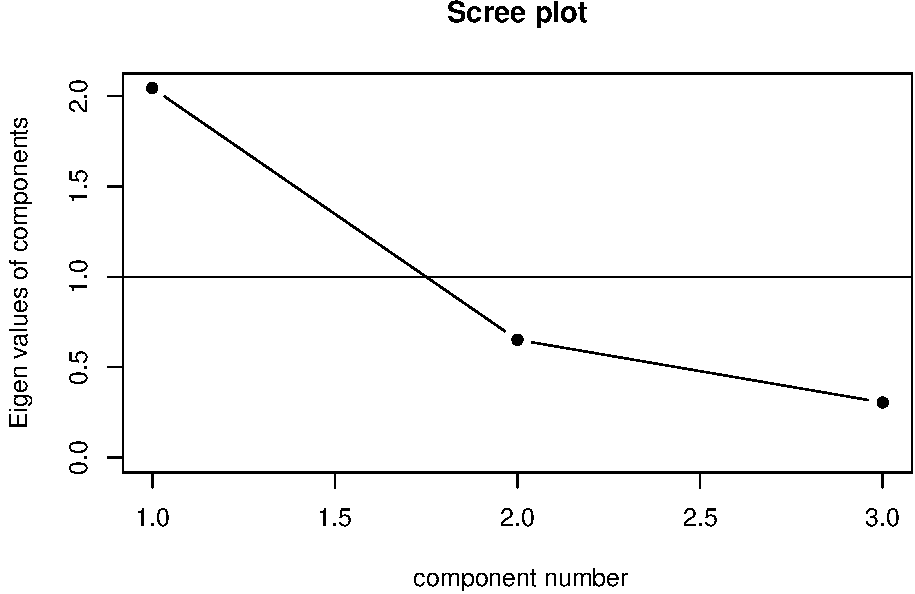
\includegraphics{PCA_covid_files/figure-latex/unnamed-chunk-35-1.pdf}

The scree plot suggests a 1 component solution. This is consistent with
the components extracted by SK from the full dataset.

\hypertarget{pca-1-component-3}{%
\subsection{PCA: 1 component}\label{pca-1-component-3}}

\begin{table}[H]

\caption{\label{tab:unnamed-chunk-36}Variance accounted for by components}
\centering
\fontsize{6}{8}\selectfont
\begin{tabular}[t]{rrlll}
\toprule
component & eigen & prop\_var & cum\_var & rotation\_SS\_load\\
\midrule
1 & 2.04 & 0.68 & 0.68 & 2.04\\
2 & 0.65 &  &  & \\
3 & 0.30 &  &  & \\
\bottomrule
\end{tabular}
\end{table}

\begin{table}[H]

\caption{\label{tab:unnamed-chunk-36}Pattern Matrix}
\centering
\fontsize{6}{8}\selectfont
\begin{tabular}[t]{lrr}
\toprule
var & PC1 & h2\\
\midrule
Govt\_Satisfaction & 0.90 & 0.82\\
Govt\_Truth & 0.79 & 0.63\\
Govt\_Extreme & -0.77 & 0.60\\
\bottomrule
\end{tabular}
\end{table}

\newpage

\hypertarget{intelligence}{%
\section{Intelligence}\label{intelligence}}

\hypertarget{correlations-between-variables-7}{%
\subsection{Correlations between
variables}\label{correlations-between-variables-7}}

\begin{table}[H]

\caption{\label{tab:unnamed-chunk-37}Correlations between variables}
\centering
\fontsize{6}{8}\selectfont
\begin{tabular}[t]{lll}
\toprule
  & 1 & 2\\
\midrule
1. CRT\_acc &  & \\
2. belief\_acc & .51** & \\
3. EAT\_acc & .53** & .58**\\
\bottomrule
\end{tabular}
\end{table}

\hypertarget{reliability-6}{%
\subsection{Reliability}\label{reliability-6}}

\begin{table}[H]

\caption{\label{tab:unnamed-chunk-38}Cronbach's Alpha}
\centering
\fontsize{6}{8}\selectfont
\begin{tabular}[t]{r}
\toprule
a\\
\midrule
0.76\\
\bottomrule
\end{tabular}
\end{table}

\hypertarget{kmo-and-bartletts-test-of-spherecity-7}{%
\subsection{KMO and Bartlett's test of
spherecity}\label{kmo-and-bartletts-test-of-spherecity-7}}

\begin{table}[H]

\caption{\label{tab:unnamed-chunk-39}KMO: Measure of sampling adequacy}
\centering
\fontsize{6}{8}\selectfont
\begin{tabular}[t]{r}
\toprule
KMO\\
\midrule
0.7\\
\bottomrule
\end{tabular}
\end{table}

\begin{table}[H]

\caption{\label{tab:unnamed-chunk-39}Bartletts test of spherecity}
\centering
\fontsize{6}{8}\selectfont
\begin{tabular}[t]{rrr}
\toprule
chisq & p.value & df\\
\midrule
375 & 0 & 3\\
\bottomrule
\end{tabular}
\end{table}

\hypertarget{scree-plot-7}{%
\subsection{Scree plot}\label{scree-plot-7}}

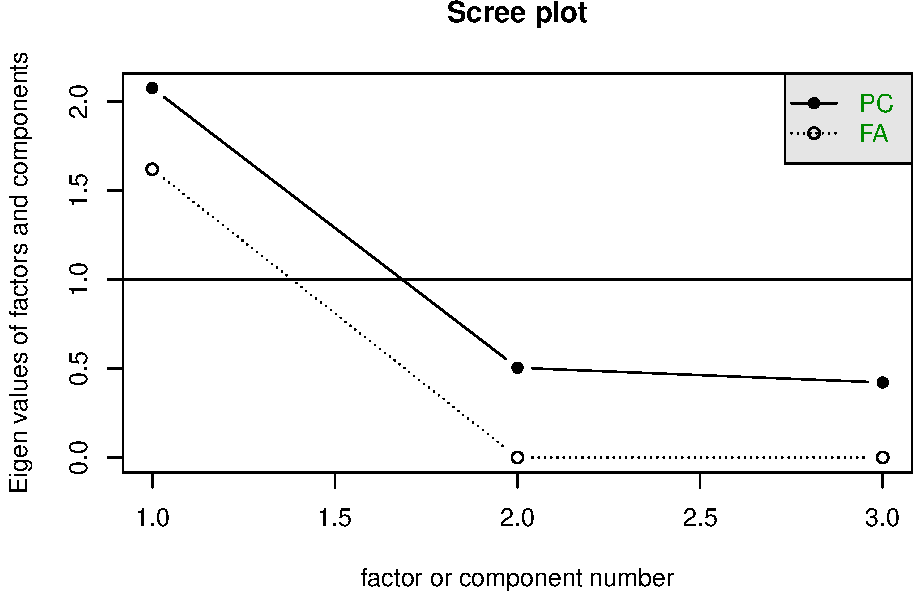
\includegraphics{PCA_covid_files/figure-latex/unnamed-chunk-40-1.pdf}

\hypertarget{pca-2}{%
\subsection{PCA}\label{pca-2}}

The scree plot suggests a 1 component solution. This is consistent with
the components extracted by SK from the full dataset.

\hypertarget{pca-1-component-4}{%
\subsection{PCA: 1 component}\label{pca-1-component-4}}

\begin{table}[H]

\caption{\label{tab:unnamed-chunk-41}Variance accounted for by components}
\centering
\fontsize{6}{8}\selectfont
\begin{tabular}[t]{rrlll}
\toprule
component & eigen & prop\_var & cum\_var & rotation\_SS\_load\\
\midrule
1 & 2.08 & 0.69 & 0.69 & 2.08\\
2 & 0.50 &  &  & \\
3 & 0.42 &  &  & \\
\bottomrule
\end{tabular}
\end{table}

\begin{table}[H]

\caption{\label{tab:unnamed-chunk-41}Pattern Matrix}
\centering
\fontsize{6}{8}\selectfont
\begin{tabular}[t]{lrr}
\toprule
var & PC1 & h2\\
\midrule
EAT\_acc & 0.85 & 0.72\\
belief\_acc & 0.84 & 0.70\\
CRT\_acc & 0.81 & 0.66\\
\bottomrule
\end{tabular}
\end{table}

\newpage

\hypertarget{news-sources}{%
\section{News sources}\label{news-sources}}

\hypertarget{correlations-between-variables-8}{%
\subsection{Correlations between
variables}\label{correlations-between-variables-8}}

\begin{table}[H]

\caption{\label{tab:unnamed-chunk-42}Correlations between variables}
\centering
\fontsize{6}{8}\selectfont
\begin{tabular}[t]{lllllll}
\toprule
  & 1 & 2 & 3 & 4 & 5 & 6\\
\midrule
1. NS\_FriendsFam &  &  &  &  &  & \\
2. NS\_OffGovt & .09** &  &  &  &  & \\
3. NS\_OffHealth & .07* & .59** &  &  &  & \\
4. NS\_Science & .02 & .35** & .50** &  &  & \\
5. NS\_WordMouth & .54** & .03 & .00 & -.02 &  & \\
\addlinespace
6. NS\_News & .15** & .13** & .00 & .04 & .20** & \\
7. NS\_SocialMedia & .31** & .08** & .07* & .05 & .38** & .23**\\
\bottomrule
\end{tabular}
\end{table}

\hypertarget{reliability-7}{%
\subsection{Reliability}\label{reliability-7}}

\begin{table}[H]

\caption{\label{tab:unnamed-chunk-43}Cronbach's Alpha}
\centering
\fontsize{6}{8}\selectfont
\begin{tabular}[t]{r}
\toprule
a\\
\midrule
0.61\\
\bottomrule
\end{tabular}
\end{table}

\hypertarget{kmo-and-bartletts-test-of-spherecity-8}{%
\subsection{KMO and Bartlett's test of
spherecity}\label{kmo-and-bartletts-test-of-spherecity-8}}

\begin{table}[H]

\caption{\label{tab:unnamed-chunk-44}KMO: Measure of sampling adequacy}
\centering
\fontsize{6}{8}\selectfont
\begin{tabular}[t]{r}
\toprule
KMO\\
\midrule
0.64\\
\bottomrule
\end{tabular}
\end{table}

\begin{table}[H]

\caption{\label{tab:unnamed-chunk-44}Bartletts test of spherecity}
\centering
\fontsize{6}{8}\selectfont
\begin{tabular}[t]{rrr}
\toprule
chisq & p.value & df\\
\midrule
1828 & 0 & 21\\
\bottomrule
\end{tabular}
\end{table}

\hypertarget{scree-plot-8}{%
\subsection{Scree plot}\label{scree-plot-8}}

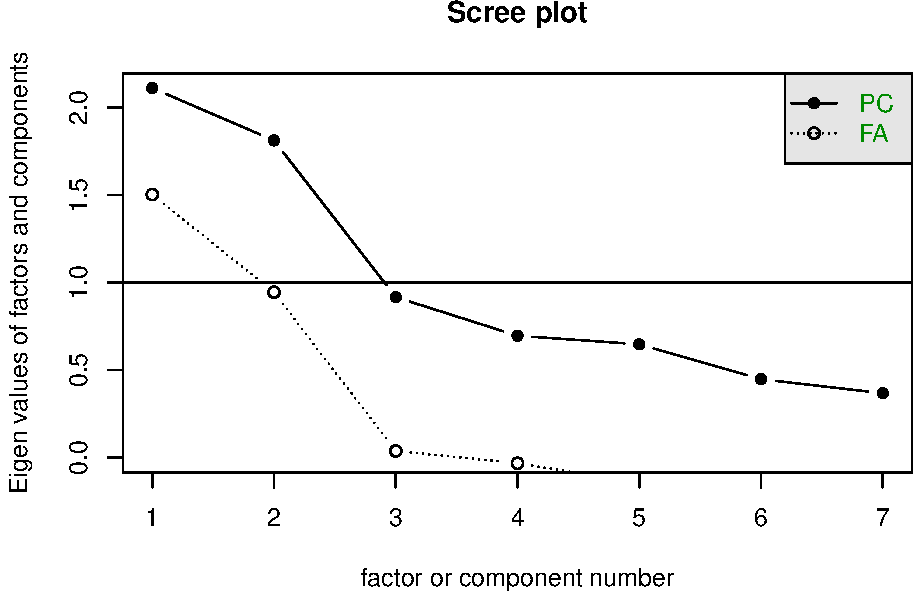
\includegraphics{PCA_covid_files/figure-latex/unnamed-chunk-45-1.pdf}

The scree plot suggests a 2 component solution. This is consistent with
the components extracted by SK from the full dataset.

\hypertarget{pca-2-component}{%
\subsection{PCA: 2 component}\label{pca-2-component}}

\begin{table}[H]

\caption{\label{tab:unnamed-chunk-46}Variance accounted for by components}
\centering
\fontsize{6}{8}\selectfont
\begin{tabular}[t]{rrlll}
\toprule
component & eigen & prop\_var & cum\_var & rotation\_SS\_load\\
\midrule
1 & 2.11 & 0.28 & 0.28 & 1.97\\
2 & 1.81 & 0.28 & 0.56 & 1.95\\
3 & 0.92 &  &  & \\
4 & 0.70 &  &  & \\
5 & 0.65 &  &  & \\
\addlinespace
6 & 0.45 &  &  & \\
7 & 0.37 &  &  & \\
\bottomrule
\end{tabular}
\end{table}

\begin{table}[H]

\caption{\label{tab:unnamed-chunk-46}Pattern Matrix}
\centering
\fontsize{6}{8}\selectfont
\begin{tabular}[t]{lllr}
\toprule
var & PC1 & PC2 & h2\\
\midrule
NS\_OffHealth & 0.88 &  & 0.76\\
NS\_OffGovt & 0.8 &  & 0.65\\
NS\_Science & 0.75 &  & 0.56\\
NS\_WordMouth &  & 0.82 & 0.67\\
NS\_FriendsFam &  & 0.77 & 0.59\\
\addlinespace
NS\_SocialMedia &  & 0.69 & 0.48\\
NS\_News &  & 0.46 & 0.22\\
\bottomrule
\end{tabular}
\end{table}

\begin{table}[H]

\caption{\label{tab:unnamed-chunk-46}Correlations between components}
\centering
\fontsize{6}{8}\selectfont
\begin{tabular}[t]{lrr}
\toprule
  & RC1 & RC2\\
\midrule
RC1 & 1.0 & 0.1\\
RC2 & 0.1 & 1.0\\
\bottomrule
\end{tabular}
\end{table}

\newpage

\hypertarget{opinion}{%
\section{Opinion}\label{opinion}}

\hypertarget{correlations-between-variables-9}{%
\subsection{Correlations between
variables}\label{correlations-between-variables-9}}

\begin{table}[H]

\caption{\label{tab:unnamed-chunk-47}Correlations between variables}
\centering
\fontsize{6}{8}\selectfont
\begin{tabular}[t]{llllllllll}
\toprule
  & 1 & 2 & 3 & 4 & 5 & 6 & 7 & 8 & 9\\
\midrule
1. opinion\_1 &  &  &  &  &  &  &  &  & \\
2. opinion\_2 & .47** &  &  &  &  &  &  &  & \\
3. opinion\_3 & .41** & .48** &  &  &  &  &  &  & \\
4. opinion\_4 & .38** & .22** & .21** &  &  &  &  &  & \\
5. opinion\_5 & -.10** & -.04 & -.04 & -.09** &  &  &  &  & \\
\addlinespace
6. opinion\_6 & -.36** & -.21** & -.19** & -.27** & .19** &  &  &  & \\
7. opinion\_7 & .50** & .33** & .35** & .54** & -.12** & -.34** &  &  & \\
8. opinion\_8 & .29** & .10** & .19** & .40** & -.06* & -.14** & .46** &  & \\
9. opinion\_9 & .31** & .35** & .34** & .28** & -.05 & -.17** & .41** & .27** & \\
10. opinion\_10 & -.20** & -.18** & -.12** & -.16** & .20** & .33** & -.26** & -.11** & -.17**\\
\bottomrule
\end{tabular}
\end{table}

\hypertarget{reliability-8}{%
\subsection{Reliability}\label{reliability-8}}

\begin{verbatim}
## Warning in psych::alpha(x): Some items were negatively correlated with the total scale and probably 
## should be reversed.  
## To do this, run the function again with the 'check.keys=TRUE' option
\end{verbatim}

\begin{verbatim}
## Some items ( opinion_5 opinion_6 opinion_10 ) were negatively correlated with the total scale and 
## probably should be reversed.  
## To do this, run the function again with the 'check.keys=TRUE' option
\end{verbatim}

\begin{table}[H]

\caption{\label{tab:unnamed-chunk-48}Cronbach's Alpha}
\centering
\fontsize{6}{8}\selectfont
\begin{tabular}[t]{r}
\toprule
a\\
\midrule
0.5\\
\bottomrule
\end{tabular}
\end{table}

\hypertarget{kmo-and-bartletts-test-of-spherecity-9}{%
\subsection{KMO and Bartlett's test of
spherecity}\label{kmo-and-bartletts-test-of-spherecity-9}}

\begin{table}[H]

\caption{\label{tab:unnamed-chunk-49}KMO: Measure of sampling adequacy}
\centering
\fontsize{6}{8}\selectfont
\begin{tabular}[t]{r}
\toprule
KMO\\
\midrule
0.83\\
\bottomrule
\end{tabular}
\end{table}

\begin{table}[H]

\caption{\label{tab:unnamed-chunk-49}Bartletts test of spherecity}
\centering
\fontsize{6}{8}\selectfont
\begin{tabular}[t]{rrr}
\toprule
chisq & p.value & df\\
\midrule
2890 & 0 & 45\\
\bottomrule
\end{tabular}
\end{table}

\hypertarget{scree-plot-9}{%
\subsection{Scree plot}\label{scree-plot-9}}

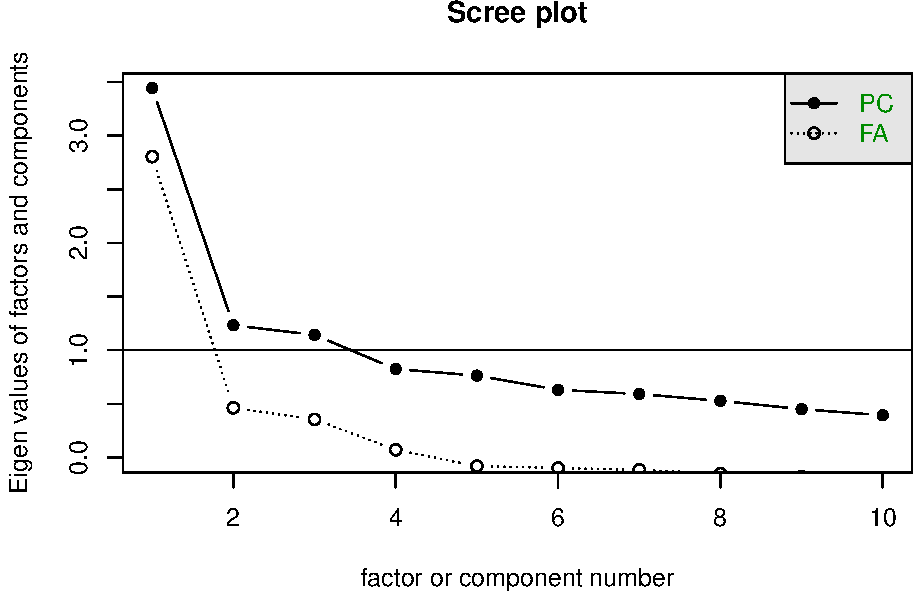
\includegraphics{PCA_covid_files/figure-latex/unnamed-chunk-50-1.pdf}

The scree plot suggests a 3 component solution. This is consistent with
the components extracted by SK from the full dataset.

\hypertarget{pca-3-component-1}{%
\subsection{PCA: 3 component}\label{pca-3-component-1}}

\begin{table}[H]

\caption{\label{tab:unnamed-chunk-51}Variance accounted for by components}
\centering
\fontsize{6}{8}\selectfont
\begin{tabular}[t]{rrlll}
\toprule
component & eigen & prop\_var & cum\_var & rotation\_SS\_load\\
\midrule
1 & 3.44 & 0.22 & 0.22 & 2.17\\
2 & 1.23 & 0.21 & 0.43 & 2.11\\
3 & 1.14 & 0.15 & 0.58 & 1.54\\
4 & 0.82 &  &  & \\
5 & 0.76 &  &  & \\
\addlinespace
6 & 0.63 &  &  & \\
7 & 0.59 &  &  & \\
8 & 0.53 &  &  & \\
9 & 0.45 &  &  & \\
10 & 0.39 &  &  & \\
\bottomrule
\end{tabular}
\end{table}

\begin{table}[H]

\caption{\label{tab:unnamed-chunk-51}Pattern Matrix}
\centering
\fontsize{6}{8}\selectfont
\begin{tabular}[t]{llllr}
\toprule
var & PC1 & PC2 & PC3 & h2\\
\midrule
opinion\_2 & 0.93 &  &  & 0.71\\
opinion\_3 & 0.85 &  &  & 0.62\\
opinion\_1 & 0.54 &  &  & 0.57\\
opinion\_9 & 0.48 &  &  & 0.42\\
opinion\_8 &  & 0.95 &  & 0.67\\
\addlinespace
opinion\_4 &  & 0.82 &  & 0.62\\
opinion\_7 &  & 0.68 &  & 0.69\\
opinion\_5 &  &  & 0.74 & 0.49\\
opinion\_10 &  &  & 0.73 & 0.53\\
opinion\_6 &  &  & 0.64 & 0.52\\
\bottomrule
\end{tabular}
\end{table}

\begin{table}[H]

\caption{\label{tab:unnamed-chunk-51}Correlations between components}
\centering
\fontsize{6}{8}\selectfont
\begin{tabular}[t]{lrrr}
\toprule
  & RC1 & RC3 & RC2\\
\midrule
RC1 & 1.00 & 0.53 & -0.32\\
RC3 & 0.53 & 1.00 & -0.34\\
RC2 & -0.32 & -0.34 & 1.00\\
\bottomrule
\end{tabular}
\end{table}

\newpage

\hypertarget{org-statements}{%
\section{Org statements}\label{org-statements}}

\hypertarget{correlations-between-variables-10}{%
\subsection{Correlations between
variables}\label{correlations-between-variables-10}}

\begin{table}[H]

\caption{\label{tab:unnamed-chunk-52}Correlations between variables}
\centering
\fontsize{6}{8}\selectfont
\begin{tabular}[t]{llll}
\toprule
  & 1 & 2 & 3\\
\midrule
1. WFH\_OrgStatements\_1 &  &  & \\
2. WFH\_OrgStatements\_2 & .43** &  & \\
3. WFH\_OrgStatements\_3 & .15** & .34** & \\
4. WFH\_OrgStatements\_4 & .22** & .46** & .66**\\
\bottomrule
\end{tabular}
\end{table}

\hypertarget{reliability-9}{%
\subsection{Reliability}\label{reliability-9}}

\begin{table}[H]

\caption{\label{tab:unnamed-chunk-53}Cronbach's Alpha}
\centering
\fontsize{6}{8}\selectfont
\begin{tabular}[t]{r}
\toprule
a\\
\midrule
0.71\\
\bottomrule
\end{tabular}
\end{table}

\hypertarget{kmo-and-bartletts-test-of-spherecity-10}{%
\subsection{KMO and Bartlett's test of
spherecity}\label{kmo-and-bartletts-test-of-spherecity-10}}

\begin{table}[H]

\caption{\label{tab:unnamed-chunk-54}KMO: Measure of sampling adequacy}
\centering
\fontsize{6}{8}\selectfont
\begin{tabular}[t]{r}
\toprule
KMO\\
\midrule
0.63\\
\bottomrule
\end{tabular}
\end{table}

\begin{table}[H]

\caption{\label{tab:unnamed-chunk-54}Bartletts test of spherecity}
\centering
\fontsize{6}{8}\selectfont
\begin{tabular}[t]{rrr}
\toprule
chisq & p.value & df\\
\midrule
407 & 0 & 6\\
\bottomrule
\end{tabular}
\end{table}

\hypertarget{scree-plot-10}{%
\subsection{Scree plot}\label{scree-plot-10}}

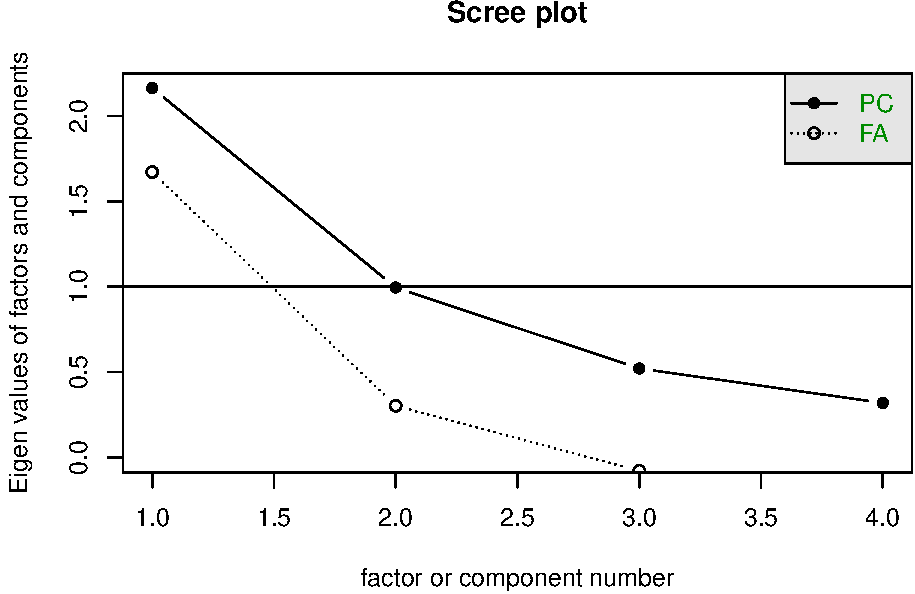
\includegraphics{PCA_covid_files/figure-latex/unnamed-chunk-55-1.pdf}

The scree plot suggests a 1 or 2 component solution. SK extracted 1
component using the full dataset so I will do the same.

\hypertarget{pca-1-component-5}{%
\subsection{PCA: 1 component}\label{pca-1-component-5}}

\begin{table}[H]

\caption{\label{tab:unnamed-chunk-56}Variance accounted for by components}
\centering
\fontsize{6}{8}\selectfont
\begin{tabular}[t]{rrlll}
\toprule
component & eigen & prop\_var & cum\_var & rotation\_SS\_load\\
\midrule
1 & 2.16 & 0.54 & 0.54 & 2.16\\
2 & 1.00 &  &  & \\
3 & 0.52 &  &  & \\
4 & 0.32 &  &  & \\
\bottomrule
\end{tabular}
\end{table}

\begin{table}[H]

\caption{\label{tab:unnamed-chunk-56}Pattern Matrix}
\centering
\fontsize{6}{8}\selectfont
\begin{tabular}[t]{lrr}
\toprule
var & PC1 & h2\\
\midrule
WFH\_OrgStatements\_4 & 0.84 & 0.71\\
WFH\_OrgStatements\_3 & 0.77 & 0.60\\
WFH\_OrgStatements\_2 & 0.76 & 0.57\\
WFH\_OrgStatements\_1 & 0.53 & 0.29\\
\bottomrule
\end{tabular}
\end{table}

\newpage

\hypertarget{reasons-to-leave}{%
\section{Reasons to leave}\label{reasons-to-leave}}

\hypertarget{correlations-between-variables-11}{%
\subsection{Correlations between
variables}\label{correlations-between-variables-11}}

\begin{table}[H]

\caption{\label{tab:unnamed-chunk-57}Correlations between variables}
\centering
\fontsize{6}{8}\selectfont
\begin{tabular}[t]{lllllllllll}
\toprule
  & 1 & 2 & 3 & 4 & 5 & 6 & 7 & 8 & 9 & 10\\
\midrule
1. ReasonsLeaveHome\_1 &  &  &  &  &  &  &  &  &  & \\
2. ReasonsLeaveHome\_2 & .03 &  &  &  &  &  &  &  &  & \\
3. ReasonsLeaveHome\_3 & .05 & .10** &  &  &  &  &  &  &  & \\
4. ReasonsLeaveHome\_4 & .06 & .11** & .23** &  &  &  &  &  &  & \\
5. ReasonsLeaveHome\_5 & .01 & .09* & .12** & .28** &  &  &  &  &  & \\
\addlinespace
6. ReasonsLeaveHome\_6 & -.02 & .04 & -.02 & -.04 & .20** &  &  &  &  & \\
7. ReasonsLeaveHome\_7 & .08* & .00 & .09** & .15** & .20** & .15** &  &  &  & \\
8. ReasonsLeaveHome\_8 & .14** & .08* & .13** & .22** & .09* & .04 & .12** &  &  & \\
9. ReasonsLeaveHome\_9 & .06 & .04 & .07 & .13** & .18** & .23** & .19** & .29** &  & \\
10. ReasonsLeaveHome\_10 & .02 & -.01 & .26** & .20** & .12** & .04 & .17** & .22** & .12** & \\
\addlinespace
11. ReasonsLeaveHome\_11 & .04 & .00 & .27** & .21** & .14** & .03 & .15** & .26** & .21** & .56**\\
\bottomrule
\end{tabular}
\end{table}

\hypertarget{reliability-10}{%
\subsection{Reliability}\label{reliability-10}}

\begin{table}[H]

\caption{\label{tab:unnamed-chunk-58}Cronbach's Alpha}
\centering
\fontsize{6}{8}\selectfont
\begin{tabular}[t]{r}
\toprule
a\\
\midrule
0.56\\
\bottomrule
\end{tabular}
\end{table}

\hypertarget{kmo-and-bartletts-test-of-spherecity-11}{%
\subsection{KMO and Bartlett's test of
spherecity}\label{kmo-and-bartletts-test-of-spherecity-11}}

\begin{table}[H]

\caption{\label{tab:unnamed-chunk-59}KMO: Measure of sampling adequacy}
\centering
\fontsize{6}{8}\selectfont
\begin{tabular}[t]{r}
\toprule
KMO\\
\midrule
0.69\\
\bottomrule
\end{tabular}
\end{table}

\begin{table}[H]

\caption{\label{tab:unnamed-chunk-59}Bartletts test of spherecity}
\centering
\fontsize{6}{8}\selectfont
\begin{tabular}[t]{rrr}
\toprule
chisq & p.value & df\\
\midrule
905 & 0 & 55\\
\bottomrule
\end{tabular}
\end{table}

\hypertarget{scree-plot-11}{%
\subsection{Scree plot}\label{scree-plot-11}}

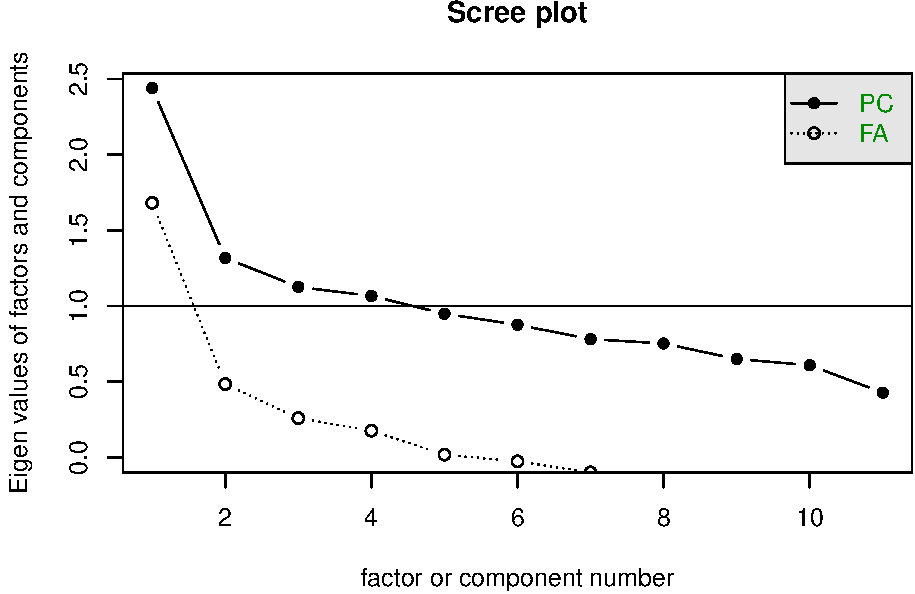
\includegraphics{PCA_covid_files/figure-latex/unnamed-chunk-60-1.pdf}

The scree plot suggests a 3 or 4 component solution. SK extracted 3
componentsusing the full dataset so I will do the same.

\hypertarget{pca-3-component-2}{%
\subsection{PCA: 3 component}\label{pca-3-component-2}}

\begin{table}[H]

\caption{\label{tab:unnamed-chunk-61}Variance accounted for by components}
\centering
\fontsize{6}{8}\selectfont
\begin{tabular}[t]{rrlll}
\toprule
component & eigen & prop\_var & cum\_var & rotation\_SS\_load\\
\midrule
1 & 2.44 & 0.18 & 0.18 & 1.96\\
2 & 1.32 & 0.14 & 0.32 & 1.54\\
3 & 1.13 & 0.13 & 0.44 & 1.38\\
4 & 1.07 &  &  & \\
5 & 0.95 &  &  & \\
\addlinespace
6 & 0.88 &  &  & \\
7 & 0.78 &  &  & \\
8 & 0.75 &  &  & \\
9 & 0.65 &  &  & \\
10 & 0.61 &  &  & \\
\addlinespace
11 & 0.43 &  &  & \\
\bottomrule
\end{tabular}
\end{table}

\begin{table}[H]

\caption{\label{tab:unnamed-chunk-61}Pattern Matrix}
\centering
\fontsize{6}{8}\selectfont
\begin{tabular}[t]{llllr}
\toprule
var & PC1 & PC2 & PC3 & h2\\
\midrule
ReasonsLeaveHome\_10 & 0.89 &  &  & 0.68\\
ReasonsLeaveHome\_11 & 0.89 &  &  & 0.69\\
ReasonsLeaveHome\_3 & 0.42 &  & 0.36 & 0.40\\
ReasonsLeaveHome\_8 & 0.33 &  &  & 0.30\\
ReasonsLeaveHome\_2 & -0.39 &  & 0.79 & 0.49\\
\addlinespace
ReasonsLeaveHome\_6 &  & 0.8 &  & 0.57\\
ReasonsLeaveHome\_9 &  & 0.62 &  & 0.45\\
ReasonsLeaveHome\_7 &  & 0.49 &  & 0.31\\
ReasonsLeaveHome\_5 &  & 0.47 & 0.37 & 0.41\\
ReasonsLeaveHome\_4 &  &  & 0.61 & 0.47\\
\addlinespace
ReasonsLeaveHome\_1 &  &  & 0.37 & 0.11\\
\bottomrule
\end{tabular}
\end{table}

\begin{table}[H]

\caption{\label{tab:unnamed-chunk-61}Correlations between components}
\centering
\fontsize{6}{8}\selectfont
\begin{tabular}[t]{lrrr}
\toprule
  & RC1 & RC2 & RC3\\
\midrule
RC1 & 1.00 & 0.27 & 0.44\\
RC2 & 0.27 & 1.00 & 0.26\\
RC3 & 0.44 & 0.26 & 1.00\\
\bottomrule
\end{tabular}
\end{table}

\newpage

\hypertarget{social-behaviour}{%
\section{Social behaviour}\label{social-behaviour}}

\hypertarget{correlations-between-variables-12}{%
\subsection{Correlations between
variables}\label{correlations-between-variables-12}}

\begin{table}[H]

\caption{\label{tab:unnamed-chunk-62}Correlations between variables}
\centering
\fontsize{6}{8}\selectfont
\begin{tabular}[t]{llllllll}
\toprule
  & 1 & 2 & 3 & 4 & 5 & 6 & 7\\
\midrule
1. BehaviourProsocial\_1 &  &  &  &  &  &  & \\
2. BehaviourProsocial\_2 & .20** &  &  &  &  &  & \\
3. BehaviourProsocial\_3 & .15** & .22** &  &  &  &  & \\
4. BehaviourProsocial\_4 & .25** & .30** & .33** &  &  &  & \\
5. BehaviourAntisocial\_1 & .11** & .08** & .11** & .11** &  &  & \\
\addlinespace
6. BehaviourAntisocial\_2 & .17** & .13** & .13** & .20** & .55** &  & \\
7. BehaviourAntisocial\_3 & .14** & .08** & .14** & .16** & .15** & .21** & \\
8. BehaviourAntisocial\_4 & .24** & .17** & .04 & .15** & .14** & .21** & .22**\\
\bottomrule
\end{tabular}
\end{table}

\hypertarget{reliability-11}{%
\subsection{Reliability}\label{reliability-11}}

\begin{table}[H]

\caption{\label{tab:unnamed-chunk-63}Cronbach's Alpha}
\centering
\fontsize{6}{8}\selectfont
\begin{tabular}[t]{r}
\toprule
a\\
\midrule
0.63\\
\bottomrule
\end{tabular}
\end{table}

\hypertarget{kmo-and-bartletts-test-of-spherecity-12}{%
\subsection{KMO and Bartlett's test of
spherecity}\label{kmo-and-bartletts-test-of-spherecity-12}}

\begin{table}[H]

\caption{\label{tab:unnamed-chunk-64}KMO: Measure of sampling adequacy}
\centering
\fontsize{6}{8}\selectfont
\begin{tabular}[t]{r}
\toprule
KMO\\
\midrule
0.68\\
\bottomrule
\end{tabular}
\end{table}

\begin{table}[H]

\caption{\label{tab:unnamed-chunk-64}Bartletts test of spherecity}
\centering
\fontsize{6}{8}\selectfont
\begin{tabular}[t]{rrr}
\toprule
chisq & p.value & df\\
\midrule
1271 & 0 & 28\\
\bottomrule
\end{tabular}
\end{table}

\hypertarget{scree-plot-12}{%
\subsection{Scree plot}\label{scree-plot-12}}

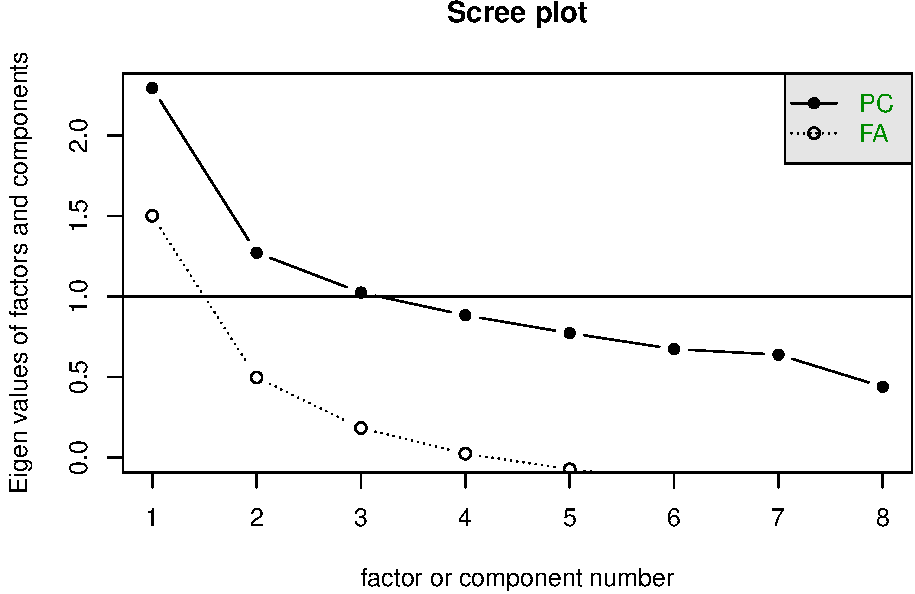
\includegraphics{PCA_covid_files/figure-latex/unnamed-chunk-65-1.pdf}

The scree plot suggests a 3 component solution. This is not consistent
with the 2 components extracted by SK from the full dataset. I will
extract 2 components only.

\hypertarget{pca-2-component-1}{%
\subsection{PCA: 2 component}\label{pca-2-component-1}}

\begin{table}[H]

\caption{\label{tab:unnamed-chunk-66}Variance accounted for by components}
\centering
\fontsize{6}{8}\selectfont
\begin{tabular}[t]{rrlll}
\toprule
component & eigen & prop\_var & cum\_var & rotation\_SS\_load\\
\midrule
1 & 2.30 & 0.23 & 0.23 & 1.85\\
2 & 1.27 & 0.21 & 0.45 & 1.72\\
3 & 1.02 &  &  & \\
4 & 0.88 &  &  & \\
5 & 0.77 &  &  & \\
\addlinespace
6 & 0.67 &  &  & \\
7 & 0.64 &  &  & \\
8 & 0.44 &  &  & \\
\bottomrule
\end{tabular}
\end{table}

\begin{table}[H]

\caption{\label{tab:unnamed-chunk-66}Pattern Matrix}
\centering
\fontsize{6}{8}\selectfont
\begin{tabular}[t]{lllr}
\toprule
var & PC1 & PC2 & h2\\
\midrule
BehaviourProsocial\_4 & 0.75 &  & 0.54\\
BehaviourProsocial\_2 & 0.7 &  & 0.44\\
BehaviourProsocial\_3 & 0.66 &  & 0.39\\
BehaviourProsocial\_1 & 0.53 &  & 0.32\\
BehaviourAntisocial\_1 &  & 0.88 & 0.69\\
\addlinespace
BehaviourAntisocial\_2 &  & 0.86 & 0.72\\
BehaviourAntisocial\_3 &  & 0.36 & 0.23\\
BehaviourAntisocial\_4 &  & 0.32 & 0.25\\
\bottomrule
\end{tabular}
\end{table}

\begin{table}[H]

\caption{\label{tab:unnamed-chunk-66}Correlations between components}
\centering
\fontsize{6}{8}\selectfont
\begin{tabular}[t]{lrr}
\toprule
  & RC1 & RC2\\
\midrule
RC1 & 1.00 & 0.37\\
RC2 & 0.37 & 1.00\\
\bottomrule
\end{tabular}
\end{table}

\newpage

\hypertarget{covid-worry}{%
\section{Covid worry}\label{covid-worry}}

\hypertarget{correlations-between-variables-13}{%
\subsection{Correlations between
variables}\label{correlations-between-variables-13}}

\begin{table}[H]

\caption{\label{tab:unnamed-chunk-67}Correlations between variables}
\centering
\fontsize{6}{8}\selectfont
\begin{tabular}[t]{lllll}
\toprule
  & 1 & 2 & 3 & 4\\
\midrule
1. CovidWorry\_1 &  &  &  & \\
2. CovidWorry\_2R & .51** &  &  & \\
3. CovidWorry\_3 & .39** & .24** &  & \\
4. CovidWorry\_4 & .39** & .23** & .47** & \\
5. CovidWorry\_5 & .51** & .35** & .46** & .42**\\
\bottomrule
\end{tabular}
\end{table}

\hypertarget{reliability-12}{%
\subsection{Reliability}\label{reliability-12}}

\begin{table}[H]

\caption{\label{tab:unnamed-chunk-68}Cronbach's Alpha}
\centering
\fontsize{6}{8}\selectfont
\begin{tabular}[t]{r}
\toprule
a\\
\midrule
0.77\\
\bottomrule
\end{tabular}
\end{table}

\hypertarget{kmo-and-bartletts-test-of-spherecity-13}{%
\subsection{KMO and Bartlett's test of
spherecity}\label{kmo-and-bartletts-test-of-spherecity-13}}

\begin{table}[H]

\caption{\label{tab:unnamed-chunk-69}KMO: Measure of sampling adequacy}
\centering
\fontsize{6}{8}\selectfont
\begin{tabular}[t]{r}
\toprule
KMO\\
\midrule
0.78\\
\bottomrule
\end{tabular}
\end{table}

\begin{table}[H]

\caption{\label{tab:unnamed-chunk-69}Bartletts test of spherecity}
\centering
\fontsize{6}{8}\selectfont
\begin{tabular}[t]{rrr}
\toprule
chisq & p.value & df\\
\midrule
1657 & 0 & 10\\
\bottomrule
\end{tabular}
\end{table}

\hypertarget{scree-plot-13}{%
\subsection{Scree plot}\label{scree-plot-13}}

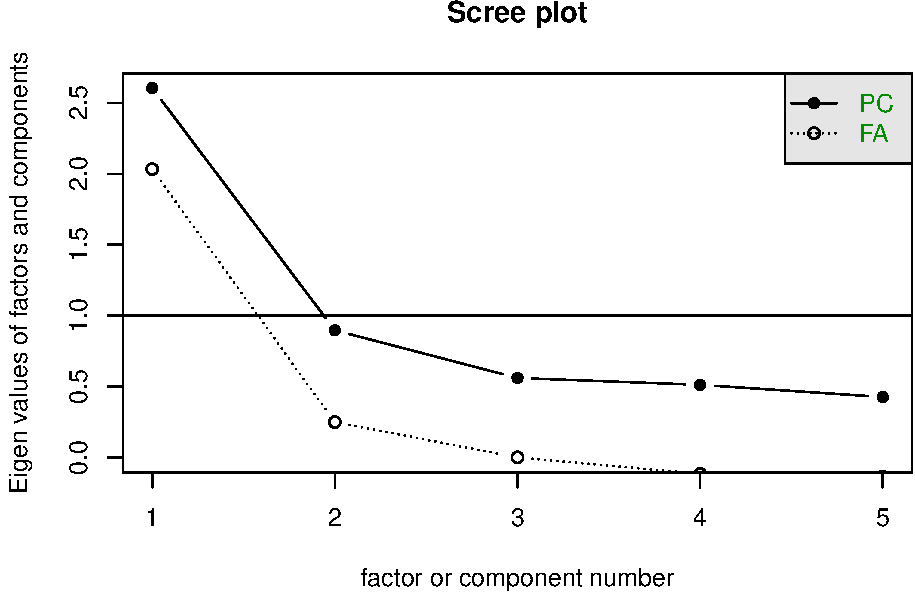
\includegraphics{PCA_covid_files/figure-latex/unnamed-chunk-70-1.pdf}

The scree plot suggests a 1 component solution. This is consistent with
the components extracted by SK from the full dataset.

\hypertarget{pca-3-component-3}{%
\subsection{PCA: 3 component}\label{pca-3-component-3}}

\begin{table}[H]

\caption{\label{tab:unnamed-chunk-71}Variance accounted for by components}
\centering
\fontsize{6}{8}\selectfont
\begin{tabular}[t]{rrlll}
\toprule
component & eigen & prop\_var & cum\_var & rotation\_SS\_load\\
\midrule
1 & 2.60 & 0.52 & 0.52 & 2.6\\
2 & 0.90 &  &  & \\
3 & 0.56 &  &  & \\
4 & 0.51 &  &  & \\
5 & 0.43 &  &  & \\
\bottomrule
\end{tabular}
\end{table}

\begin{table}[H]

\caption{\label{tab:unnamed-chunk-71}Pattern Matrix}
\centering
\fontsize{6}{8}\selectfont
\begin{tabular}[t]{lrr}
\toprule
var & PC1 & h2\\
\midrule
CovidWorry\_1 & 0.79 & 0.63\\
CovidWorry\_5 & 0.77 & 0.60\\
CovidWorry\_3 & 0.71 & 0.51\\
CovidWorry\_4 & 0.69 & 0.48\\
CovidWorry\_2R & 0.63 & 0.39\\
\bottomrule
\end{tabular}
\end{table}

\end{document}
